\begin{frame}{What SHAP Consumes and Produces}

    \centering
    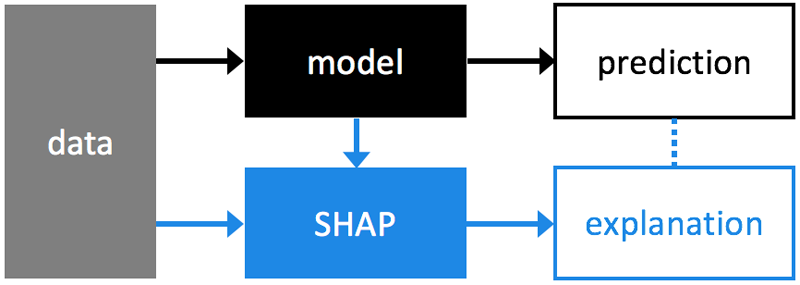
\includegraphics[width=0.50\textwidth,height=0.34\textheight,keepaspectratio]{images/responsible-ai/shap_pipeline_diagram.png}

    \vspace{0.3em}
    {\scriptsize Source: \texttt{shap} library documentation artwork,
    \href{https://github.com/shap/shap}{github.com/shap/shap} (\texttt{docs/artwork/shap\_diagram.png}).}

    \vspace{0.7em}
    \raggedright
    \begin{itemize}\small
        \setlength\itemsep{0.3em}
        \item SHAP does not change the model. It takes the \textbf{fitted model} plus a
              \textbf{background dataset} and produces one attribution per feature per row.
        \item The background dataset defines $\mathbb{E}[f(X)]$ --- the reference the explanation is
              measured against. \textbf{Change the background and every number changes}, so record
              which rows you used.
        \item A useful phrasing for stakeholders: \emph{``compared with a typical applicant, this
              applicant's income pushed the score up by 0.31.''}
    \end{itemize}
\end{frame}

\begin{frame}{Local View: The Waterfall Plot}

    \centering
    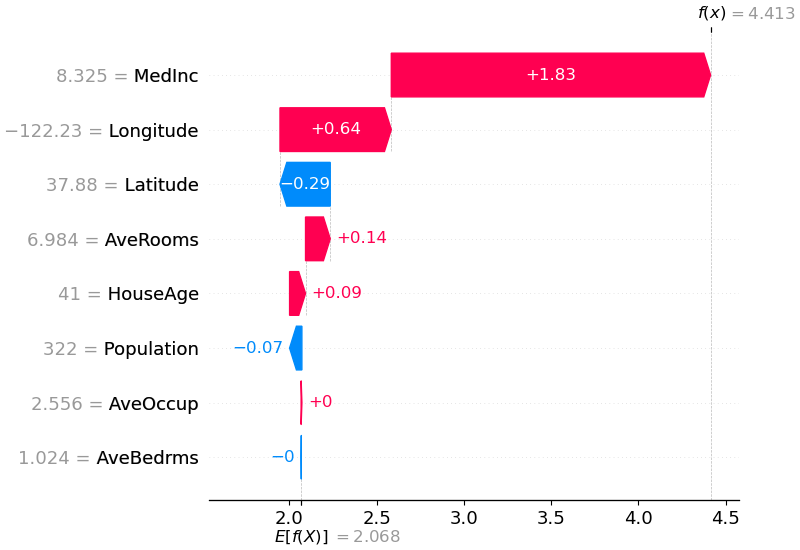
\includegraphics[width=0.60\textwidth,height=0.42\textheight,keepaspectratio]{images/responsible-ai/shap_waterfall_california.png}

    \vspace{0.3em}
    {\scriptsize Source: \texttt{shap} library documentation artwork,
    \href{https://github.com/shap/shap}{github.com/shap/shap}
    (\texttt{docs/artwork/california\_waterfall.png}); model trained on the California Housing
    dataset, target in units of \$100k.}

    \vspace{0.6em}
    \raggedright
    \begin{itemize}\small
        \setlength\itemsep{0.3em}
        \item Read bottom to top: start at the base value $\mathbb{E}[f(X)] = 2.068$, add each
              feature's contribution, arrive at this row's prediction $f(x) = 4.413$.
        \item The grey number on the left is the feature's actual value for this row.
        \item This is the artefact to show a domain expert. One row, one story, and it adds up.
    \end{itemize}
\end{frame}

\begin{frame}{Global View: The Beeswarm Summary Plot}

    \centering
    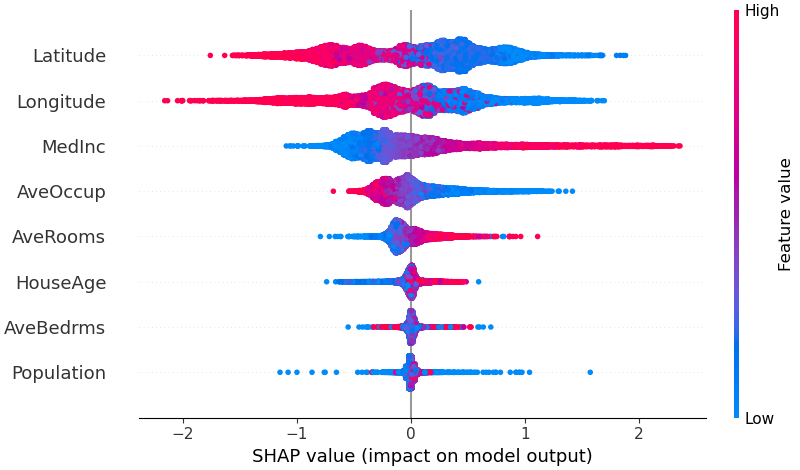
\includegraphics[width=0.58\textwidth,height=0.42\textheight,keepaspectratio]{images/responsible-ai/shap_beeswarm_california.png}

    \vspace{0.3em}
    {\scriptsize Source: \texttt{shap} library documentation artwork,
    \href{https://github.com/shap/shap}{github.com/shap/shap}
    (\texttt{docs/artwork/california\_beeswarm.png}).}

    \vspace{0.5em}
    \raggedright
    \begin{itemize}\small
        \setlength\itemsep{0.3em}
        \item One dot per row per feature; horizontal position is the SHAP value, colour is the
              \textbf{feature value} (red high, blue low). Features are ordered by mean $|\phi|$.
        \item Read the \textbf{direction}: for \texttt{MedInc}, red dots sit on the right, so higher
              median income pushes the predicted price up --- monotone and sensible.
        \item Read the \textbf{spread}: a feature with a wide swarm matters a lot for some rows and
              not at all for others. A bar chart of mean $|\phi|$ would have hidden that.
    \end{itemize}
\end{frame}

\begin{frame}{Interaction View: The Dependence / Scatter Plot}

    \centering
    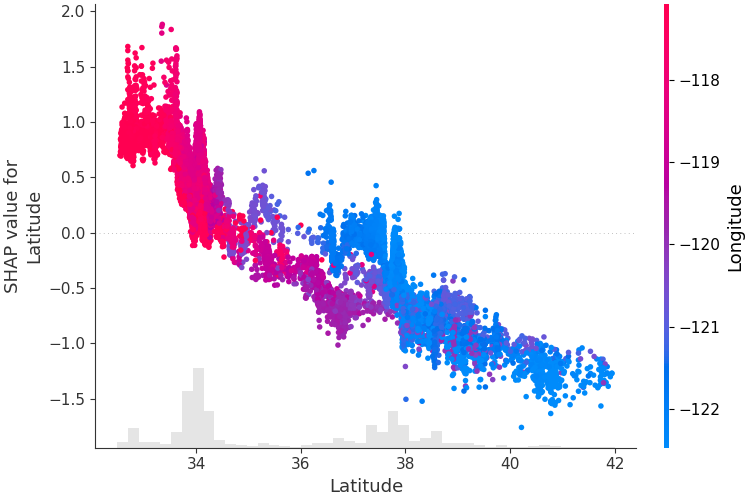
\includegraphics[width=0.47\textwidth,height=0.42\textheight,keepaspectratio]{images/responsible-ai/shap_scatter_california.png}

    \vspace{0.3em}
    {\scriptsize Source: \texttt{shap} library documentation artwork,
    \href{https://github.com/shap/shap}{github.com/shap/shap}
    (\texttt{docs/artwork/california\_scatter.png}).}

    \vspace{0.5em}
    \raggedright
    \begin{itemize}\small
        \setlength\itemsep{0.3em}
        \item $x$-axis: the feature's value. $y$-axis: its SHAP value. This is the model's learned
              response to that feature, without assuming it is linear or monotone.
        \item Colouring by a second feature exposes \textbf{interactions}: here the vertical spread
              at a given latitude is explained by longitude --- the model has learned geography,
              not a one-dimensional rule.
        \item Sharp steps are informative: they are the split points of the underlying trees.
    \end{itemize}
\end{frame}

\begin{frame}{Which SHAP Estimator?}

    \centering
    \scriptsize
    \begin{tabular}{p{2.5cm} p{4.2cm} p{5.2cm}}
        \toprule
        \textbf{Estimator} & \textbf{Applies to} & \textbf{Notes} \\
        \midrule
        \textbf{TreeSHAP} & Trees, random forests, gradient boosting (XGBoost, LightGBM, CatBoost)
        & Exact, in polynomial time, by exploiting the tree structure. Fast enough for a whole
          dataset. \textbf{Use this whenever you can.} \\
        \addlinespace
        \textbf{KernelSHAP} & Anything with \texttt{predict()}
        & Weighted local linear regression over sampled coalitions. Model-agnostic but
          \textbf{slow}; sample a few hundred background rows and a subset of instances. \\
        \addlinespace
        \textbf{DeepSHAP / Gradient} & Neural networks
        & Uses backpropagation and a DeepLIFT-style approximation; much cheaper than KernelSHAP. \\
        \addlinespace
        \textbf{Linear} & Linear models
        & Closed form: $\phi_i = w_i (x_i - \mathbb{E}[X_i])$ under feature independence. \\
        \bottomrule
    \end{tabular}

    \vspace{0.9em}
    \raggedright
    {\scriptsize Polynomial-time exact tree attribution: S.~M.~Lundberg et al., ``From local
    explanations to global understanding with explainable AI for trees,'' \emph{Nature Machine
    Intelligence} 2:56--67, 2020.}
\end{frame}

\begin{frame}{LIME: Fit a Simple Model in a Small Neighbourhood}

    \centering
    \resizebox{\textwidth}{!}{%
    \begin{tikzpicture}[
        node distance=0.75cm,
        limestep/.style={rectangle, draw, rounded corners, minimum height=1.25cm, text width=2.35cm,
                     align=center, font=\scriptsize, fill=raiBlue!10},
        arr/.style={-{Latex[length=2.2mm]}, thick}
    ]
        \node[limestep] (a) {Pick the row $x$ to explain};
        \node[limestep, right=of a] (b) {Perturb it: sample many nearby variants};
        \node[limestep, right=of b] (c) {Ask the black box to label them};
        \node[limestep, right=of c] (d) {Weight samples by closeness to $x$};
        \node[limestep, right=of d, fill=raiGreen!12] (e) {Fit a sparse linear model on the weights};

        \foreach \x/\y in {a/b, b/c, c/d, d/e} \draw[arr] (\x) -- (\y);
    \end{tikzpicture}}

    \vspace{1.0em}

    \raggedright
    \begin{itemize}
        \setlength\itemsep{0.4em}
        \item The coefficients of that little linear model \emph{are} the explanation.
        \item ``Perturb'' is domain-specific: for text, delete words; for images, switch
              superpixels on and off; for tabular data, sample around the row.
        \item The surrogate is deliberately \textbf{sparse} (a handful of features) so a human can
              read it. Complexity is traded for legibility, on purpose.
    \end{itemize}

    \vspace{0.4em}
    {\scriptsize M.~T.~Ribeiro, S.~Singh and C.~Guestrin, ``\,`Why Should I Trust You?': Explaining
    the Predictions of Any Classifier,'' KDD 2016,
    \href{https://arxiv.org/abs/1602.04938v3}{arXiv:1602.04938v3}.}
\end{frame}

\begin{frame}{LIME on Tabular Data}

    \centering
    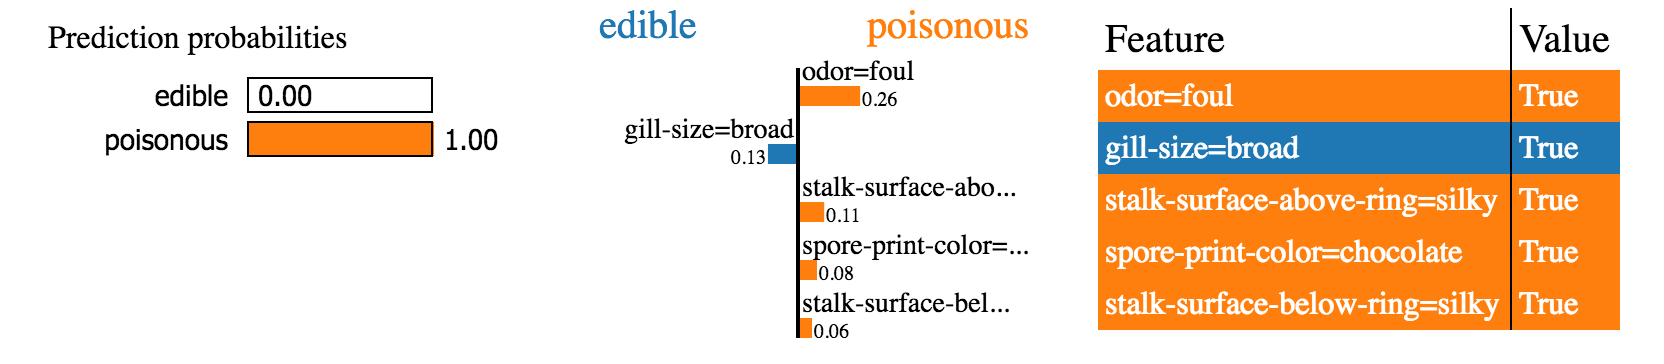
\includegraphics[width=0.92\textwidth,height=0.40\textheight,keepaspectratio]{images/responsible-ai/lime_tabular_explanation.png}

    \vspace{0.3em}
    {\scriptsize Source: \texttt{lime} library documentation,
    \href{https://github.com/marcotcr/lime}{github.com/marcotcr/lime}
    (\texttt{doc/images/tabular.png}); mushroom edibility classifier.}

    \vspace{0.7em}
    \raggedright
    \begin{itemize}\small
        \setlength\itemsep{0.3em}
        \item Left: the predicted class probabilities. Middle: signed contributions of the top
              features. Right: the actual feature values for this row.
        \item The explanation is in terms of \textbf{discretised bins}
              (\texttt{odor=foul}), which is why it reads well to a non-specialist --- and why the
              numbers depend on how you binned.
        \item Note the contrast with SHAP: LIME's weights are coefficients of a local surrogate.
              They do \textbf{not} sum to the prediction.
    \end{itemize}
\end{frame}
